\documentclass[12pt, twoside]{article}
\input{../preamble}
\usepackage{pgfplots}
\usepgfplotslibrary{fillbetween}
\pgfplotsset{compat=1.16}

\fancyhead[LE]{\thepage}
\fancyhead[RO]{Markscheme}
\fancyhead[LO]{La Scuola d'Italia / Dr.\ Huson / IB Math: Calculus \\* 14 April 2026}

\begin{document}
\subsubsection*{5.12 Classwork: Trigonometric Transformations \& Derivatives --- Markscheme}

\begin{enumerate}

%--- Problem 1: Ferris wheel [8 marks] ---
\item [Maximum mark: 8]

Ferris wheel with diameter 80\,m, lowest point 5\,m above ground, period 16 minutes.
$h(t) = a\cos(bt) + d$.

\begin{enumerate}
\item[(a)] Find $a$, $b$, $d$. \hfill [4]

Radius $= 40$, centre height $= 5 + 40 = 45$ \hfill \textbf{(A1)}

$d = 45$ \hfill \textbf{(A1)}

$a = -40$ \quad (negative: starts at minimum with cosine) \hfill \textbf{(A1)}

Period $= 16$, so $\dfrac{2\pi}{b} = 16 \Rightarrow b = \dfrac{\pi}{8}$ \hfill \textbf{(A1)}

\item[(b)] Find $h(4)$. \hfill [2]

$h(4) = -40\cos\!\left(\dfrac{\pi}{8} \cdot 4\right) + 45$ \hfill \textbf{(M1)}

$= -40\cos\!\left(\dfrac{\pi}{2}\right) + 45 = -40(0) + 45 = 45$\,m \hfill \textbf{(A1)}

\textit{The seat is at the centre height (moving through the midpoint going up).}

\item[(c)] Find $h'(t)$ and state what it represents. \hfill [2]

$h'(t) = -40 \cdot \left(-\dfrac{\pi}{8}\right)\sin\!\left(\dfrac{\pi t}{8}\right)
= 5\pi\sin\!\left(\dfrac{\pi t}{8}\right)$ \hfill \textbf{(A1)}

This represents the rate of change of height (vertical speed) in m/min. \hfill \textbf{(A1)}
\end{enumerate}
\vspace{0.5cm}

%--- Problem 2: Transformations [10 marks] ---
\item [Maximum mark: 10]

$y = 3\sin\!\left(2\!\left(x - \dfrac{\pi}{4}\right)\right) + 1$

\begin{enumerate}
\item[(a)] Describe the transformations: \hfill [4]

(i) Vertical stretch by factor 3. \hfill \textbf{(A1)}

(ii) Horizontal compression by factor $\dfrac{1}{2}$. \hfill \textbf{(A1)}

(iii) Horizontal translation $\dfrac{\pi}{4}$ units to the right. \hfill \textbf{(A1)}

(iv) Vertical translation 1 unit up. \hfill \textbf{(A1)}

\item[(b)] Write down: \hfill [2]

(i) Amplitude $= 3$ \hfill \textbf{(A1)}

(ii) Period $= \dfrac{2\pi}{2} = \pi$ \hfill \textbf{(A1)}

\item[(c)] Sketch the graph. \hfill [4]

\begin{center}
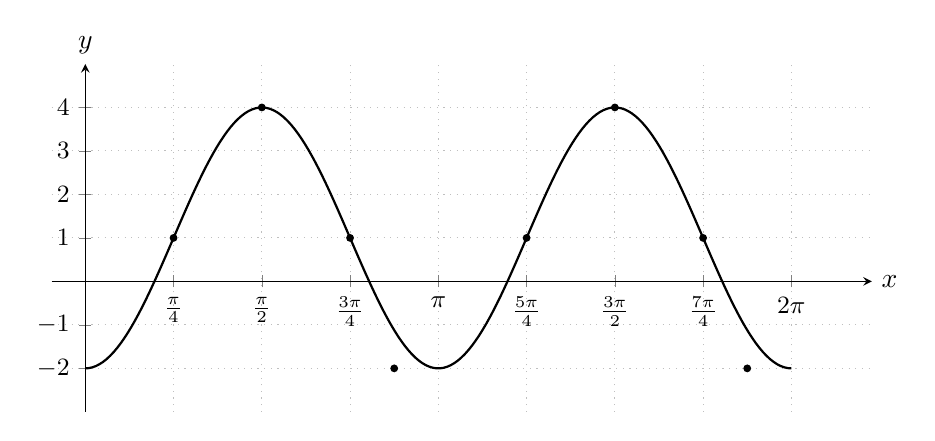
\begin{tikzpicture}
\begin{axis}[
    width=12cm, height=6cm,
    axis lines=middle,
    xlabel={$x$}, ylabel={$y$},
    xmin=-0.3, xmax=7,
    ymin=-3, ymax=5,
    xtick={0.7854, 1.5708, 2.3562, 3.1416, 3.927, 4.7124, 5.4978, 6.2832},
    xticklabels={$\frac{\pi}{4}$, $\frac{\pi}{2}$, $\frac{3\pi}{4}$, $\pi$,
      $\frac{5\pi}{4}$, $\frac{3\pi}{2}$, $\frac{7\pi}{4}$, $2\pi$},
    ytick={-2, -1, 0, 1, 2, 3, 4},
    minor y tick num=0,
    grid=major,
    grid style={dotted, gray!50},
    tick label style={font=\small},
    every axis x label/.style={at={(ticklabel* cs:1)}, anchor=west},
    every axis y label/.style={at={(ticklabel* cs:1)}, anchor=south},
]
\addplot[thick, domain=0:6.2832, samples=200]
    {3*sin(deg(2*(x - 0.7854))) + 1};
% Key points
\node[fill=black, circle, inner sep=1pt] at (axis cs:0.7854, 1) {};
\node[fill=black, circle, inner sep=1pt] at (axis cs:1.5708, 4) {};
\node[fill=black, circle, inner sep=1pt] at (axis cs:2.3562, 1) {};
\node[fill=black, circle, inner sep=1pt] at (axis cs:2.7489, -2) {};
\node[fill=black, circle, inner sep=1pt] at (axis cs:3.927, 1) {};
\node[fill=black, circle, inner sep=1pt] at (axis cs:4.7124, 4) {};
\node[fill=black, circle, inner sep=1pt] at (axis cs:5.4978, 1) {};
\node[fill=black, circle, inner sep=1pt] at (axis cs:5.8905, -2) {};
\end{axis}
\end{tikzpicture}
\end{center}

\textit{Award \textbf{(A1)} for correct shape (sinusoidal, 2 complete cycles in $[0, 2\pi]$).
\textbf{(A1)} for correct amplitude (max $= 4$, min $= -2$).
\textbf{(A1)} for correct horizontal shift (first ``mid-crossing'' at $x = \pi/4$).
\textbf{(A1)} for correct vertical shift (midline at $y = 1$).}
\end{enumerate}

\newpage

%--- Problem 3: Derivatives [7 marks] ---
\item [Maximum mark: 7]

\begin{enumerate}
\item[(a)] $f(x) = 3\sin x + 2\cos x$ \hfill [2]

$f'(x) = 3\cos x - 2\sin x$ \hfill \textbf{(A1)(A1)}

\textit{Award \textbf{(A1)} for each correct term.}

\item[(b)] $g(x) = 4\cos(3x)$ \hfill [2]

$g'(x) = 4 \cdot (-\sin(3x)) \cdot 3 = -12\sin(3x)$ \hfill \textbf{(M1)(A1)}

\textit{Award \textbf{(M1)} for applying the chain rule. \textbf{(A1)} for correct answer.}

\item[(c)] $h(x) = \sin^2 x = (\sin x)^2$ \hfill [3]

$h'(x) = 2\sin x \cdot \cos x$ \hfill \textbf{(M1)(A1)}

$= \sin 2x$ \hfill \textbf{(A1)}

\textit{Award \textbf{(M1)} for chain rule with $2(\sin x)$ as outer derivative.
\textbf{(A1)} for $\cdot\cos x$ as inner derivative. Final \textbf{(A1)} for
simplified form $\sin 2x$. Accept $2\sin x\cos x$.}
\end{enumerate}
\vspace{0.3cm}

%--- Problem 4: f(x) = 2sin(3x) - 1 [7 marks] ---
\item [Maximum mark: 7]

$f(x) = 2\sin(3x) - 1$

\begin{enumerate}
\item[(a)] Find $f'(x)$. \hfill [2]

$f'(x) = 2 \cdot 3\cos(3x) = 6\cos(3x)$ \hfill \textbf{(M1)(A1)}

\item[(b)] Find $x$-coordinates of max and min. \hfill [3]

$f'(x) = 0 \Rightarrow \cos(3x) = 0$ \hfill \textbf{(M1)}

$3x = \dfrac{\pi}{2},\, \dfrac{3\pi}{2},\, \dfrac{5\pi}{2}$
\quad $\Rightarrow$ \quad
$x = \dfrac{\pi}{6},\, \dfrac{\pi}{2},\, \dfrac{5\pi}{6}$ \hfill \textbf{(A1)}

Maximum at $x = \dfrac{\pi}{6}$ and $x = \dfrac{5\pi}{6}$;
\quad minimum at $x = \dfrac{\pi}{2}$ \hfill \textbf{(A1)}

\textit{Award final \textbf{(A1)} for correctly identifying which are maxima and which is a minimum.}

\item[(c)] Find max and min values. \hfill [2]

$f\!\left(\dfrac{\pi}{6}\right) = 2\sin\!\left(\dfrac{\pi}{2}\right) - 1
= 2(1) - 1 = 1$ \hfill \textbf{(A1)}

$f\!\left(\dfrac{\pi}{2}\right) = 2\sin\!\left(\dfrac{3\pi}{2}\right) - 1
= 2(-1) - 1 = -3$ \hfill \textbf{(A1)}

\textit{Maximum value is $1$, minimum value is $-3$.}
\end{enumerate}

\newpage

%--- Problem 5: g(x) = a sin(bx) + c [6 marks] ---
\item [Maximum mark: 6]

$g(x) = a\sin(bx) + c$, max $= 7$, min $= 1$, period $= \dfrac{2\pi}{3}$.

\begin{enumerate}
\item[(a)] Find $a$, $b$, $c$. \hfill [3]

Amplitude: $a = \dfrac{7 - 1}{2} = 3$ \hfill \textbf{(A1)}

Vertical shift: $c = \dfrac{7 + 1}{2} = 4$ \hfill \textbf{(A1)}

Period: $\dfrac{2\pi}{b} = \dfrac{2\pi}{3} \Rightarrow b = 3$ \hfill \textbf{(A1)}

\item[(b)] Find $g'\!\left(\dfrac{\pi}{6}\right)$. \hfill [3]

$g'(x) = 3 \cdot 3\cos(3x) = 9\cos(3x)$ \hfill \textbf{(M1)(A1)}

$g'\!\left(\dfrac{\pi}{6}\right) = 9\cos\!\left(\dfrac{\pi}{2}\right) = 9(0) = 0$ \hfill \textbf{(A1)}
\end{enumerate}
\vspace{0.5cm}

%--- Problem 6: cos 2x + 2sin x [6 marks] ---
\item [Maximum mark: 6]

$f(x) = \cos 2x + 2\sin x$

\begin{enumerate}
\item[(a)] Show that $f'(x) = 2\cos x(1 - 2\sin x)$. \hfill [3]

$f'(x) = -2\sin 2x + 2\cos x$ \hfill \textbf{(A1)}

$= -2(2\sin x\cos x) + 2\cos x$ \hfill \textbf{(M1)}

$= -4\sin x\cos x + 2\cos x = 2\cos x(1 - 2\sin x)$ \hfill \textbf{(AG)}

\textit{Award \textbf{(A1)} for correct differentiation. \textbf{(M1)} for using
$\sin 2x = 2\sin x\cos x$ and factoring. Must see all steps for \textbf{(AG)}.}

\item[(b)] Find values of $x$ where $f'(x) = 0$. \hfill [3]

$\cos x = 0$ \quad $\Rightarrow$ \quad $x = \dfrac{\pi}{2},\, \dfrac{3\pi}{2}$ \hfill \textbf{(A1)}

$1 - 2\sin x = 0$ \quad $\Rightarrow$ \quad $\sin x = \dfrac{1}{2}$ \hfill \textbf{(M1)}

$x = \dfrac{\pi}{6},\, \dfrac{5\pi}{6}$ \hfill \textbf{(A1)}

\textit{All four values required for full marks:
$x = \dfrac{\pi}{6},\, \dfrac{\pi}{2},\, \dfrac{5\pi}{6},\, \dfrac{3\pi}{2}$.}
\end{enumerate}

\end{enumerate}
\end{document}
